\begin{figure}[!ht]
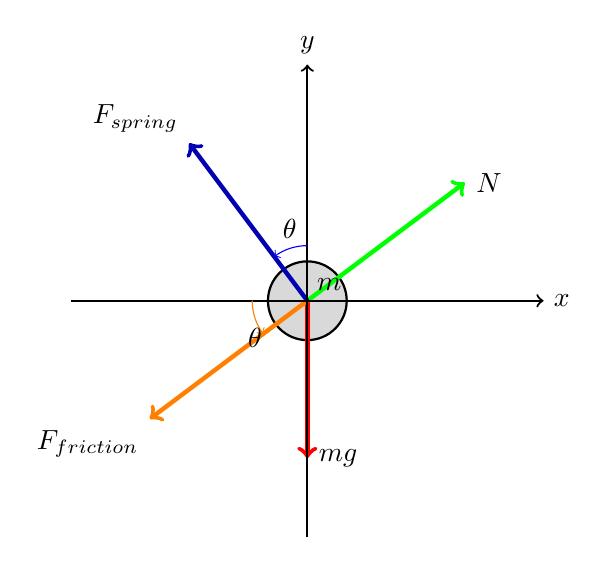
\begin{tikzpicture}
    \centering
    \draw[thick, fill=gray!30] (0,0) circle (0.5cm);
    
    \draw[->, ultra thick, green] (0,0) -- (2,1.5) node[right, black]{$N$};
    \draw[->, ultra thick, red] (0,0) -- (0,-2) node[right, black]{$mg$};
    \draw[->, ultra thick, orange] (0,0) -- (-2,-1.5) node[below left, black]{$F_{\text{friction}}$};
    \draw[->, ultra thick, blue!70!black] (0,0) -- (-1.5,2) node[above left, black]{$F_{\text{spring}}$};    
    
    \node at (0,0) [above right]{$m$};
    
    \draw[->, thick] (-3,0) -- (3,0) node[right]{$x$};
    \draw[->, thick] (0,-3) -- (0,3) node[above]{$y$};
    
    %approximated the angle to 37 degrees theta = 37 deg
    \draw[->, blue] (0,0) ++(90:0.7cm) arc (90:127:0.7cm) node[midway, above, black] {$\theta$};
    \draw[->, orange] (0,0) ++(180:0.7cm) arc (180:217:0.7cm) node[midway, below, black] {$\theta$};
\end{tikzpicture}
\caption{Maximum spring force FBD}
    \label{fig:fig1_xe80}
\end{figure}
